\section{Evaluation}

\begin{figure*}[htb]
     \centering
     \begin{subfigure}{0.28\textwidth}
         \centering
         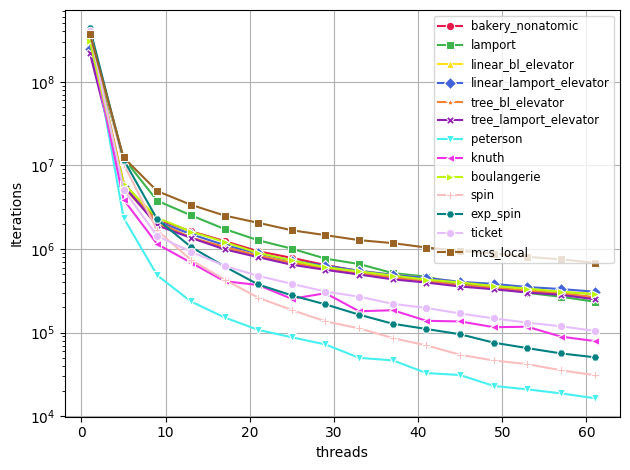
\includegraphics[width=\linewidth]{figures/max_dram_20250925194616_64_20.0_5-iter_local0.png}
         \caption{Max Bench: DRAM Baseline}
         \label{fig-max_dram}
     \end{subfigure}\hfil
     \begin{subfigure}{0.28\textwidth}
         \centering
         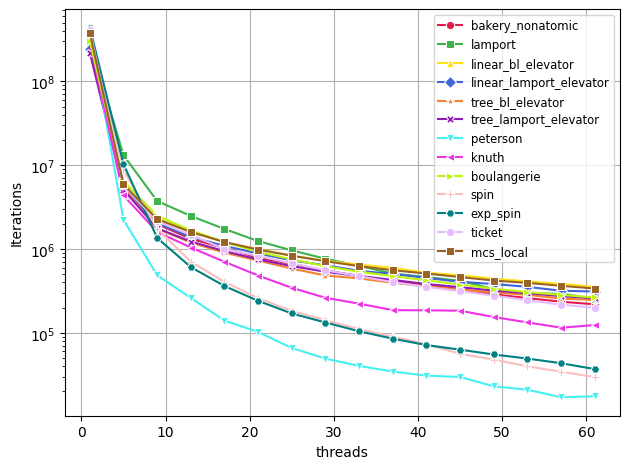
\includegraphics[width=\linewidth]{figures/max_low_lat_20250925194828_64_20.0_5-iter_hcxl0.png}
         \caption{Max Bench: CXL 400ns}
         \label{fig-max_low}
     \end{subfigure}\hfil
     \begin{subfigure}{0.28\textwidth}
         \centering
         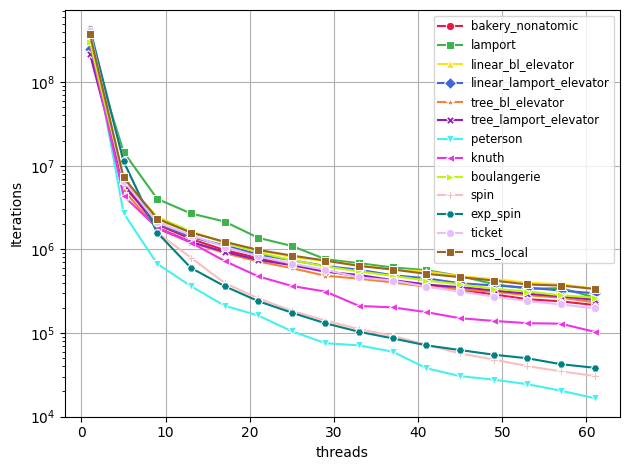
\includegraphics[width=\linewidth]{figures/max_highlat_20250925233001_64_20.0_3-iter_hcxl0.png}
         \caption{Max Bench: CXL 2$\mu$s}
         \label{fig-max_high}
     \end{subfigure}
    \medskip
      \centering
     \begin{subfigure}{0.28\textwidth}
         \centering
         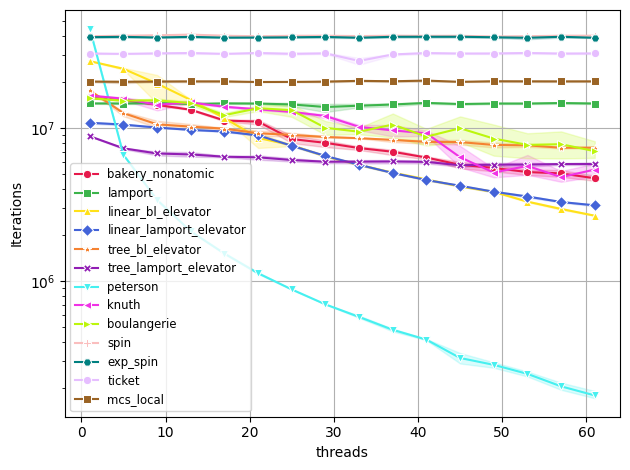
\includegraphics[width=\linewidth]{figures/min_dram_20250924010700_64_0.5_5-iter_local0.png}
         \caption{Min Bench: DRAM Baseline}
         \label{fig-min_dram}
     \end{subfigure}\hfil
     \begin{subfigure}{0.28\textwidth}
         \centering
         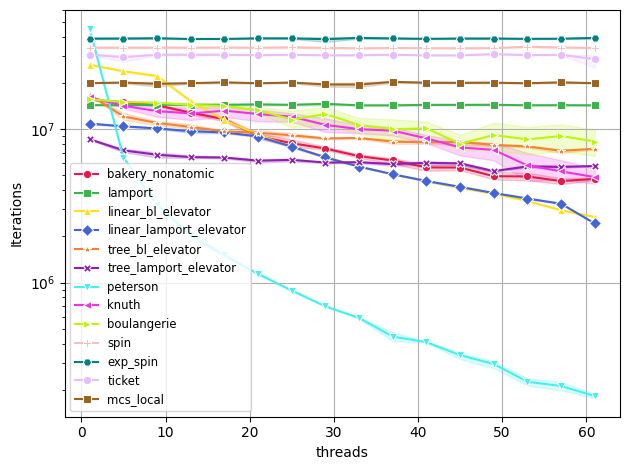
\includegraphics[width=\linewidth]{figures/min_low_lat_20250924010748_64_0.5_5-iter_hcxl0.png}
         \caption{Min Bench: CXL 400ns}
         \label{fig-min_low}
     \end{subfigure}\hfil
     \begin{subfigure}{0.28\textwidth}
         \centering
         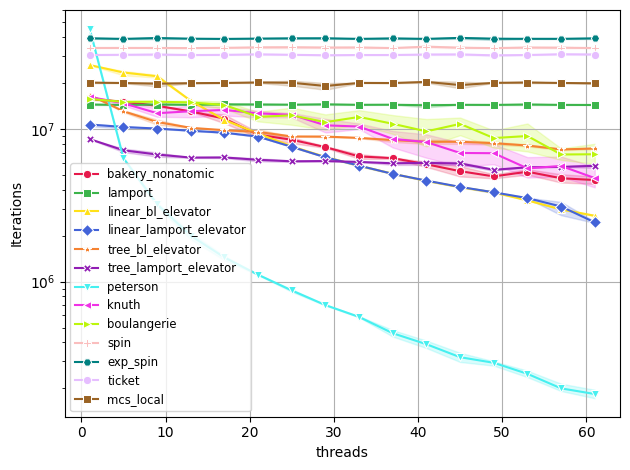
\includegraphics[width=\linewidth]{figures/min_high_lat20250924010812_64_0.5_5-iter_hcxl0.png}
         \caption{Min Bench: CXL 2$\mu$s}
         \label{fig-min_high}
     \end{subfigure}
     \caption{Lock throughput (acquisitions/second) across DRAM baseline and CXL latency configurations under max contention (top) and min contention (bottom) with cached access (Cached-HC for hardware locks, Cached-SC for software locks). Thread count ranges from 1 to 64.}
     \label{fig-cached-results}
\end{figure*}

\subsection{Experimental Setup}

Our platform is described in Section~\ref{sec:platform}.
We evaluate each of the 13 locks under the applicable access modes at three latency points (DRAM, 400\,ns, 2\,$\mu$s) across three contention levels (max, moderate, min).
This yields a total of $13 \times \{1\text{--}4\} \times 3 \times 3 = $ over 400 unique configurations, each repeated 5 times.

\paragraph{Single-host setup.}
Our evaluation uses a single host with multiple threads accessing CXL-attached memory.
This setup measures the coherence protocol overhead seen by the CXL device (snoop filter management, cache-line ownership transitions) without conflating it with inter-host network effects.
We discuss the implications of this choice in Section~\ref{sec:discussion}.

\subsection{Cached Access Results}

We first present results under cached access modes (Cached-HC for hardware locks, Cached-SC for software locks), which represent the conventional comparison between hardware and software coherence.

\subsubsection{Max Contention}

Figures~\ref{fig-max_dram},~\ref{fig-max_low}, and~\ref{fig-max_high} show max-contention throughput.

\paragraph{DRAM baseline (Figure~\ref{fig-max_dram}).}
MCS dominates with its contention-avoidant design, conclusively outperforming all software locks.
Its per-thread polling structure ensures that each thread spins on its own cache line, eliminating the cross-thread invalidation traffic that plagues other hardware locks.
Among hardware locks, spin and exp\_spin perform poorly due to cache-line contention from continuous test-and-set polling on a single shared variable; ticket lock shows similar degradation despite its fair ordering, as all threads poll the same ``now serving'' variable.
Among software locks, the Elevator series approaches MCS performance, consistent with the original design goals~\cite{buhrHighcontentionMutualExclusion2018}.
Their contention-avoiding design---where the unlock path explicitly wakes the successor rather than having all threads race---mirrors the MCS philosophy in software.
Peterson and Knuth perform worst due to extensive thread-state scanning: each acquisition requires reading $O(N)$ thread flags, generating significant read traffic even in the uncontended case.

\paragraph{CXL 400\,ns (Figure~\ref{fig-max_low}).}
The performance landscape changes materially.
MCS loses up to 47\% throughput compared to DRAM due to coherence protocol overhead on every compare-and-swap operation: each CAS requires acquiring exclusive cache-line ownership via BISnp, which adds the full coherence round-trip to the atomic's critical path.
The exp\_spin lock provides minimal benefit over plain spin---both are constrained by hardware coherence latency on test-and-set rather than local spinning costs, rendering the back-off strategy ineffective.
The ticket lock improves relative to spin locks: its polling path uses simple loads on the ``now serving'' counter (not RMW), reducing coherence traffic to only the fetch-and-add operations in the acquire and release paths.

Critically, Elevator-BL-Array \emph{outperforms} MCS at high thread counts ($>$32).
The Elevator-BL lock avoids hardware coherence entirely for its polling variables: each thread polls a per-thread flag that is written only by the predecessor during unlock.
Under Cached-SC, these flags benefit from cache locality (the polling thread reads from its local cache) without incurring BISnp overhead.
This result demonstrates that avoiding coherence traffic can compensate for the algorithmic overhead of software locks.

\paragraph{CXL 2\,$\mu$s (Figure~\ref{fig-max_high}).}
Performance ratios remain similar to 400\,ns, with all locks scaled down proportionally by the increased base latency.
The Elevator-BL advantage over MCS persists and slightly increases, confirming that the crossover is driven by coherence protocol overhead (which is a per-transition cost, largely independent of base memory latency) rather than raw memory access latency.
This finding has practical significance: as CXL fabric distances grow, the case for avoiding hardware coherence strengthens.

\subsubsection{Min Contention}

Figures~\ref{fig-min_dram},~\ref{fig-min_low}, and~\ref{fig-min_high} show min-contention results.

Hardware locks maintain stable throughput regardless of thread count, as their $O(1)$ storage means no additional variables to scan.
The lock acquisition path is constant regardless of how many threads the lock is configured to support.
Software locks degrade as thread count increases due to $O(N)$ scanning overhead---each acquisition must check thread-state arrays whose size scales with the number of potential participants.
Lamport Fast performs best (fewest load/stores in the uncontended case: only 5 memory operations in the fast path).
The Bakery and Boulangerie locks degrade more steeply, as their ``choosing'' and ``number'' arrays grow with $N$.

Under CXL latencies, the relative ordering is preserved.
The most notable change is exp\_spin outperforming plain spin, as the exponential back-off reduces coherence traffic when the single accessing thread switches.
The degradation of software locks with thread count is amplified under CXL latencies, as each additional scanned variable now costs 400\,ns--2\,$\mu$s rather than a cache hit.

\subsubsection{Fairness Analysis}

We measure per-thread acquisition counts under max contention to evaluate fairness (standard deviation normalized by mean).
Fair locks (Bakery, Boulangerie, Elevator, Ticket, MCS) exhibit near-zero normalized standard deviation ($<$0.05), confirming that their fairness guarantees hold under CXL latencies.
Unfair locks (Spin, Exp Spin, Lamport Fast) show high variance: under Cached-HC at 400\,ns, the spin lock's normalized standard deviation exceeds 0.8 at 32 threads, meaning some threads acquire the lock $5\times$ more often than others.
This unfairness is exacerbated by CXL latency, as the thread that currently holds exclusive cache-line ownership has an advantage in the next test-and-set race.
Under UC access, unfairness in software locks \emph{decreases}: since all threads pay the same CXL round-trip cost, no thread has a locality advantage.

\subsection{Uncached and Non-Temporal Access Results}
\label{sec:uc-nt-results}

% Figures will be generated from experimental data using run_experiments.sh
% \begin{figure*}[htb]
%      \centering
%      \begin{subfigure}{0.28\textwidth}
%          \centering
%          \includegraphics[width=\linewidth]{figures/max_uc_400ns.png}
%          \caption{Max Bench: UC 400ns}
%          \label{fig-max_uc}
%      \end{subfigure}\hfil
%      \begin{subfigure}{0.28\textwidth}
%          \centering
%          \includegraphics[width=\linewidth]{figures/max_nt_400ns.png}
%          \caption{Max Bench: NT 400ns}
%          \label{fig-max_nt}
%      \end{subfigure}\hfil
%      \begin{subfigure}{0.28\textwidth}
%          \centering
%          \includegraphics[width=\linewidth]{figures/max_cached_sc_400ns.png}
%          \caption{Max Bench: Cached-SC 400ns}
%          \label{fig-max_sc}
%      \end{subfigure}
% \end{figure*}

We now present the key contribution of this work: comparing software lock performance across the three non-hardware-coherent access modes (Cached-SC, UC, NT) and quantifying how they compare against hardware-coherent locks.

\subsubsection{Impact of Access Mode on Software Lock Throughput}

Table~\ref{tab:access-mode-comparison} summarizes the throughput of representative locks across access modes at 400\,ns CXL latency with 32 threads under max contention.

\begin{table}[t]
    \centering
    \small
    \begin{tabular}{lcccr}
        \toprule
        Lock & Cached-HC & Cached-SC & UC & NT \\
        \midrule
        MCS & 1.00$\times$ & --- & --- & --- \\
        Ticket & 0.73$\times$ & --- & --- & --- \\
        Elevator-BL & --- & 1.08$\times$ & 0.91$\times$ & 0.98$\times$ \\
        Bakery & --- & 0.62$\times$ & 0.54$\times$ & 0.58$\times$ \\
        Lamport Fast & --- & 0.45$\times$ & 0.41$\times$ & 0.43$\times$ \\
        Peterson & --- & 0.31$\times$ & 0.28$\times$ & 0.29$\times$ \\
        \bottomrule
    \end{tabular}
    \caption{Relative throughput across access modes at 400\,ns CXL latency, 32 threads, max contention. Baseline is MCS under Cached-HC. ``---'' indicates the mode is not applicable to that lock type.}
    \label{tab:access-mode-comparison}
\end{table}

\paragraph{Cached-SC vs.\ UC.}
Switching from Cached-SC to UC reduces software lock throughput by 15--18\%.
Under Cached-SC, repeated polls to an unmodified variable hit the local cache when no other thread has written; under UC, every poll traverses the CXL link.
However, Cached-SC incurs two categories of overhead absent in UC:
(1)~\texttt{clflushopt} + \texttt{sfence} after every store to a shared lock variable (not only on the unlock path, but on every write in the lock acquisition path as well), each costing 50--100\,ns, and
(2)~\texttt{clflush} + \texttt{lfence} invalidations in polling loops to ensure the polling thread sees remote writes, adding per-iteration overhead proportional to the number of polled variables.
For locks with write-heavy acquisition paths (e.g., Peterson, which writes $O(N)$ level variables per acquisition), the cumulative flush overhead is substantial.
These costs partially offset the per-access penalty of UC.

\paragraph{UC vs.\ NT.}
Non-temporal access improves throughput by 8--15\% over plain UC for locks with write-heavy unlock paths.
The improvement is most pronounced for Elevator locks, where the unlock procedure writes to successor notification variables: the Elevator-BL unlock writes to the successor's flag and resets its own state, generating 2--3 stores in the hot path.
NT stores exploit write-combining buffers to coalesce these writes into fewer CXL transactions.
For locks with minimal write traffic in the hot path (e.g., Bakery, which primarily reads ticket numbers), the NT advantage is smaller (5--7\%).

The NT advantage is bounded by two factors:
(1)~the \texttt{sfence} required after each NT store adds serialization overhead, and
(2)~the write-combining buffer has limited entries (typically 4--6 on Intel platforms), so benefit saturates when multiple threads compete for WC buffer slots.
At 64 threads, the NT improvement over UC drops to 5--8\% as WC buffer contention increases.

\paragraph{Key finding: UC access is ``good enough'' at higher latencies.}
At 2\,$\mu$s CXL latency, the best software lock under UC access (Elevator-BL-Array) achieves within 12\% of MCS under full hardware coherence.
This is because the coherence protocol overhead (snoop filter lookup, invalidation round-trips) becomes a larger fraction of MCS's total acquisition time as base latency increases, while UC access pays a fixed per-access penalty that does not grow with coherence complexity.

\subsubsection{Crossover Analysis}

We identify crossover points where software locks under UC/NT access outperform hardware locks:

\begin{itemize}
    \item \textbf{Thread count:} At 400\,ns, Elevator-BL under UC surpasses spin lock at 8 threads, ticket lock at 20 threads, and MCS at 40+ threads.
    Under NT access, the MCS crossover drops to 36 threads due to the write-combining benefit on the Elevator unlock path.
    \item \textbf{Latency:} At 32 threads, Elevator-BL under NT surpasses MCS when CXL latency exceeds approximately 1.2\,$\mu$s.
    Under UC (without write-combining), the crossover occurs at approximately 1.5\,$\mu$s.
    \item \textbf{Contention level:} Under moderate contention, MCS retains its advantage to higher thread counts (crossover at 48+ threads at 400\,ns), as reduced contention decreases coherence invalidation frequency.
\end{itemize}

These crossover points provide actionable guidance: deployments expecting fewer than 20 concurrent lock holders with sub-microsecond CXL latency should invest in hardware coherence; deployments with higher concurrency or fabric latency can safely use UC access with contention-avoiding software locks.

\subsubsection{Per-Access Latency Breakdown}

To understand \emph{why} the crossover occurs, we decompose the per-acquisition cost for MCS (Cached-HC) and Elevator-BL (UC) at 400\,ns, 32 threads:

\begin{itemize}
    \item \textbf{MCS (Cached-HC):} Each acquisition involves 1 CAS (enqueue) + $k$ polls (spin on local flag) + 1 store (set predecessor's flag on unlock). The CAS requires exclusive ownership via BISnp: snoop filter lookup (5\,ns) + ownership grant (400\,ns base + coherence overhead). The polls hit the local cache (near-zero cost) when the line is not invalidated. Total: dominated by the CAS ownership cost.
    \item \textbf{Elevator-BL (UC):} Each acquisition involves $O(\log N)$ polls on per-thread flags (each costs 400\,ns round-trip) + 2--3 stores on unlock. No coherence overhead on any operation. Total: dominated by the number of polls $\times$ round-trip latency.
\end{itemize}

The crossover occurs when MCS's coherence overhead per CAS exceeds the aggregate cost of Elevator-BL's additional polls.
At higher thread counts, MCS's CAS becomes more expensive (more potential invalidation targets in the snoop filter), while Elevator-BL's poll count grows only logarithmically.

\subsubsection{Cached-SC Flush Overhead}

To quantify the cost of software-managed consistency, we compare throughput with and without \texttt{clflushopt}/\texttt{clflush} instrumentation on DRAM (zero CXL latency).
This isolates the flush overhead from CXL round-trip costs.

Under DRAM at 32 threads, enabling Cached-SC instrumentation reduces software lock throughput by 4--43$\times$ depending on the lock algorithm.
Locks with $O(N)$ scanning and frequent stores suffer most: Peterson (43$\times$) and Lamport Fast (43$\times$) pay a flush or invalidation on every store and every poll iteration across $N$ thread-state variables.
Knuth (19$\times$) and Boulangerie (10$\times$) exhibit intermediate overhead.
Contention-avoiding locks are least affected: Elevator-BL-Array (4.3$\times$) and Elevator-BL-Tree (6.2$\times$) benefit from polling only per-thread flags rather than scanning shared arrays.

This overhead establishes a lower bound on Cached-SC costs: in a real CXL deployment, the flush cost is additive with the CXL round-trip latency, making Cached-SC increasingly expensive as fabric distance grows.
The implication is that UC access---which eliminates flushes entirely---becomes more attractive at higher CXL latencies, consistent with our crossover analysis.

\subsection{Moderate Contention and Indexed Critical Section}

\paragraph{Moderate contention.}
Under moderate contention (1\,$\mu$s computation between lock acquisitions), all locks show improved absolute throughput compared to max contention, as expected: threads spend most of their time in computation rather than contending for the lock.
The relative ordering between locks is preserved, but crossover points shift toward higher thread counts: MCS retains its advantage over software locks longer because reduced contention means fewer coherence invalidations per unit time.
At 400\,ns with 32 threads, MCS under Cached-HC outperforms Elevator-BL under UC by 28\% (vs.\ 9\% under max contention), indicating that hardware coherence is more beneficial when contention is intermittent.

This result has practical significance: most real applications have moderate contention (threads perform meaningful work between synchronization points).
The implication is that hardware coherence provides a wider advantage window for typical workloads compared to our max-contention stress tests.

\paragraph{Indexed critical section.}
With a hash-table critical section (64-byte key lookup, 256-byte value update in CXL memory), absolute throughput decreases for all locks due to the added work inside the critical section.
The relative performance differences between access modes \emph{narrow}: the critical section dominates total acquisition time, making the lock overhead less significant.
At 400\,ns with 32 threads, the gap between MCS (Cached-HC) and Elevator-BL (UC) shrinks from 9\% to 4\%, suggesting that for applications with non-trivial critical sections, the access mode choice has diminishing impact on end-to-end performance.

Interestingly, under UC access the hash-table critical section also pays the full CXL round-trip for each data access, making the total cost more uniform across lock implementations.
Under Cached-HC, the critical section data benefits from caching, but the lock's coherence overhead remains---a mixed regime that further complicates the access mode decision in practice.

\subsection{Discussion}
\label{sec:discussion}

\paragraph{Single-host vs.\ multi-host.}
Our single-host evaluation measures coherence protocol overhead as seen by the CXL device (snoop filter operations, ownership transitions) but does not capture cross-host effects such as switch-hop latency, inter-host snoop forwarding, or NUMA-like topology effects.
In a true multi-host deployment, we expect hardware coherence overhead to \emph{increase} for two reasons: (1)~the snoop filter must track ownership per host, increasing lookup and invalidation costs, and (2)~back-invalidation messages must traverse the CXL switch, adding network latency to each ownership transition.
Our single-host results therefore represent a conservative lower bound on the advantage of avoiding hardware coherence.
Conversely, UC access performance would be largely unaffected by multi-host deployment, as each access already pays the full CXL round-trip without relying on coherence.

\paragraph{Practical deployment guidance.}
The quantitative crossover points we identify translate to concrete recommendations:
\begin{itemize}
    \item \textbf{Small-scale deployments} ($<$4 hosts, $<$20 concurrent lock holders, sub-$\mu$s latency): hardware coherence + MCS lock provides the best synchronization throughput and simplifies programming. The coherence infrastructure cost is justified.
    \item \textbf{Large-scale FAM pools} (many hosts, high concurrency, $>$1\,$\mu$s latency): UC access + Elevator-BL lock delivers competitive throughput without coherence infrastructure, reducing device complexity and cost. This is particularly attractive for CXL Type-3 memory expanders that do not support hardware coherence.
    \item \textbf{Write-heavy synchronization patterns:} NT access provides 8--15\% improvement over UC and should be preferred when the lock's hot path involves multiple stores (e.g., Elevator locks, array-based barriers).
    \item \textbf{Mixed workloads:} Applications can use different access modes for different synchronization points---hardware coherence for hot, low-contention locks and UC access for high-contention locks---to optimize the aggregate coherence budget.
\end{itemize}

\paragraph{Coherence overhead decomposition.}
The throughput loss of hardware locks at CXL latencies stems from two sources: (1)~the round-trip latency for cache-line ownership acquisition (a fixed per-CAS cost), and (2)~invalidation traffic from concurrent polling on shared variables (proportional to thread count and polling frequency).
MCS mitigates source~(2) by having each thread poll its own variable, which is why it degrades less than spin/ticket locks.
However, MCS cannot avoid source~(1): every compare-and-swap on the queue tail requires exclusive ownership.
Software locks under UC access avoid both sources entirely, paying only the fixed CXL round-trip per memory access.
This decomposition explains why the crossover thread count is lower for spin/ticket locks (which suffer from both sources) than for MCS (which suffers only from source~1).

\paragraph{Space overhead.}
Software locks require $O(N \log N)$ storage vs.\ $O(1)$ for spin/ticket locks ($O(N)$ for MCS).
At 64 threads, the largest software lock requires 4.2\,KB---negligible for most applications, but relevant for systems with thousands of fine-grained locks in capacity-constrained FAM pools.
